\documentclass[12pt, oneside]{book}
\usepackage[utf8]{inputenc}
\usepackage{graphicx}
\usepackage[slovak]{babel}
\usepackage{todonotes}
\usepackage{url}
\usepackage{listings}
\usepackage{longtable}
\usepackage{pdflscape}
\usepackage{graphicx}
\usepackage{indentfirst}
\linespread{1.3}
\usepackage{chngcntr}
\counterwithout{footnote}{chapter}

\lstdefinestyle{customBash}{
  belowcaptionskip=1\baselineskip,
  breaklines=true,
  frame=L,
  xleftmargin=\parindent,
  language=bash,
  showstringspaces=false,
  basicstyle=\footnotesize\ttfamily,
  keywordstyle=\bfseries\color{green!40!black},
  commentstyle=\itshape\color{purple!40!black},
  identifierstyle=\color{blue},
  stringstyle=\color{red},
}

\lstdefinestyle{customC}{
  belowcaptionskip=1\baselineskip,
  breaklines=true,
  frame=L,
  xleftmargin=\parindent,
  language=c,
  showstringspaces=false,
  basicstyle=\footnotesize\ttfamily,
  keywordstyle=\bfseries\color{green!40!black},
  commentstyle=\itshape\color{purple!40!black},
  identifierstyle=\color{blue},
  stringstyle=\color{red},
}

\colorlet{punct}{red!60!black}
\definecolor{background}{HTML}{EEEEEE}
\definecolor{delim}{RGB}{20,105,176}
\colorlet{numb}{magenta!60!black}

\lstdefinelanguage{json}{
    basicstyle=\normalfont\ttfamily,
    numbers=left,
    numberstyle=\scriptsize,
    stepnumber=1,
    numbersep=8pt,
    showstringspaces=false,
    breaklines=true,
    frame=lines,
    backgroundcolor=\color{background},
    literate=
     *{0}{{{\color{numb}0}}}{1}
      {1}{{{\color{numb}1}}}{1}
      {2}{{{\color{numb}2}}}{1}
      {3}{{{\color{numb}3}}}{1}
      {4}{{{\color{numb}4}}}{1}
      {5}{{{\color{numb}5}}}{1}
      {6}{{{\color{numb}6}}}{1}
      {7}{{{\color{numb}7}}}{1}
      {8}{{{\color{numb}8}}}{1}
      {9}{{{\color{numb}9}}}{1}
      {:}{{{\color{punct}{:}}}}{1}
      {,}{{{\color{punct}{,}}}}{1}
      {\{}{{{\color{delim}{\{}}}}{1}
      {\}}{{{\color{delim}{\}}}}}{1}
      {[}{{{\color{delim}{[}}}}{1}
      {]}{{{\color{delim}{]}}}}{1},
}


\setcounter{secnumdepth}{3}
\setcounter{tocdepth}{3}

% -------------------
% --- Definicia zakladnych pommov
% -------------------
\def\*{{\bf FIXME: }}
\def\mfyear{2015}
\def\mftitle{Použitie honey-pot-u na analýzu prihlasovacích údajov používaných pri útokoch}
\def\mfthesistype{bakalárska práca}
\def\mfauthor{Tomáš Kubla}
\def\mfadvisor{RNDr. Jaroslav Janáček PhD.}
\def\mfplacedate{Bratislava, \mfyear}
\def\odbor{2508 Informatika} %aj cislo odboru je povinne a je to podla katedry/odboru, na ktorom je autor
\def\program{ Informatika }
\def\stredisko{ Katedra informatiky }

\begin{document}     

% -------------------
% --- Obalka ------
% -------------------
\thispagestyle{empty}
\noindent

\begin{minipage}{0.95\textwidth}
\begin{center}
\sc  
\large
\vspace*{0.3cm} Univerzita Komenského v Bratislave\\
\vspace*{0.3cm} Fakulta matematiky, fyziky a informatiky\\
\end{center}
\end{minipage}

\vfill

\begin{minipage}{1.1\textwidth}
\begin{flushright}
\bigskip\bigskip
% tusim mam nadstandardne dlhy nazov :)
%\centerline{\sc\LARGE\mftitle}
\begin{center}
\sc\LARGE\mftitle
\end{center}
\bigskip
\centerline{\sc\mfthesistype}

\bigskip\bigskip\bigskip\bigskip
\end{flushright}
\end{minipage}
\vfill

\noindent \mfyear\\
\indent\mfauthor

\eject % EOP i
% --- koniec obalky ----

% -------------------
% --- Titulný list
% -------------------

\thispagestyle{empty}
\noindent

\begin{minipage}{0.95\textwidth}
\begin{center}
\sc  
\large
\vspace*{0.3cm} Univerzita Komenského v Bratislave\\
\vspace*{0.3cm} Fakulta matematiky, fyziky a informatiky\\
\end{center}
\end{minipage}

\vfill

\begin{minipage}{1.1\textwidth}
\begin{flushright}
\bigskip\bigskip
% tusim mam nadstandardne dlhy nazov :)
%\centerline{\sc\LARGE\mftitle}
\begin{center}
\sc\LARGE\mftitle
\end{center}
\bigskip
\centerline{\sc\mfthesistype}
\end{flushright}

\bigskip
\vspace{3cm}
\bigskip
\begin{tabular}{ll}
Študijný program: & \program \\
Študijný odbor: & \odbor \\
Školiace pracovisko: & \stredisko \\
Školiteľ: & \mfadvisor \\
\end{tabular}

\end{minipage}
\vfill

\noindent \mfplacedate\\
\indent\mfauthor

\eject % EOP i


% --- Koniec titulnej strany


% -------------------
% --- Naskenovane Zadanie
% -------------------
% v tlačenej verzii s podpismi zainteresovaných osôb.
% v elektronickej verzii sa zverejňuje zadanie bez podpisov zainteresovaných osôb.

\newpage 
\thispagestyle{empty}
\hspace{-3cm}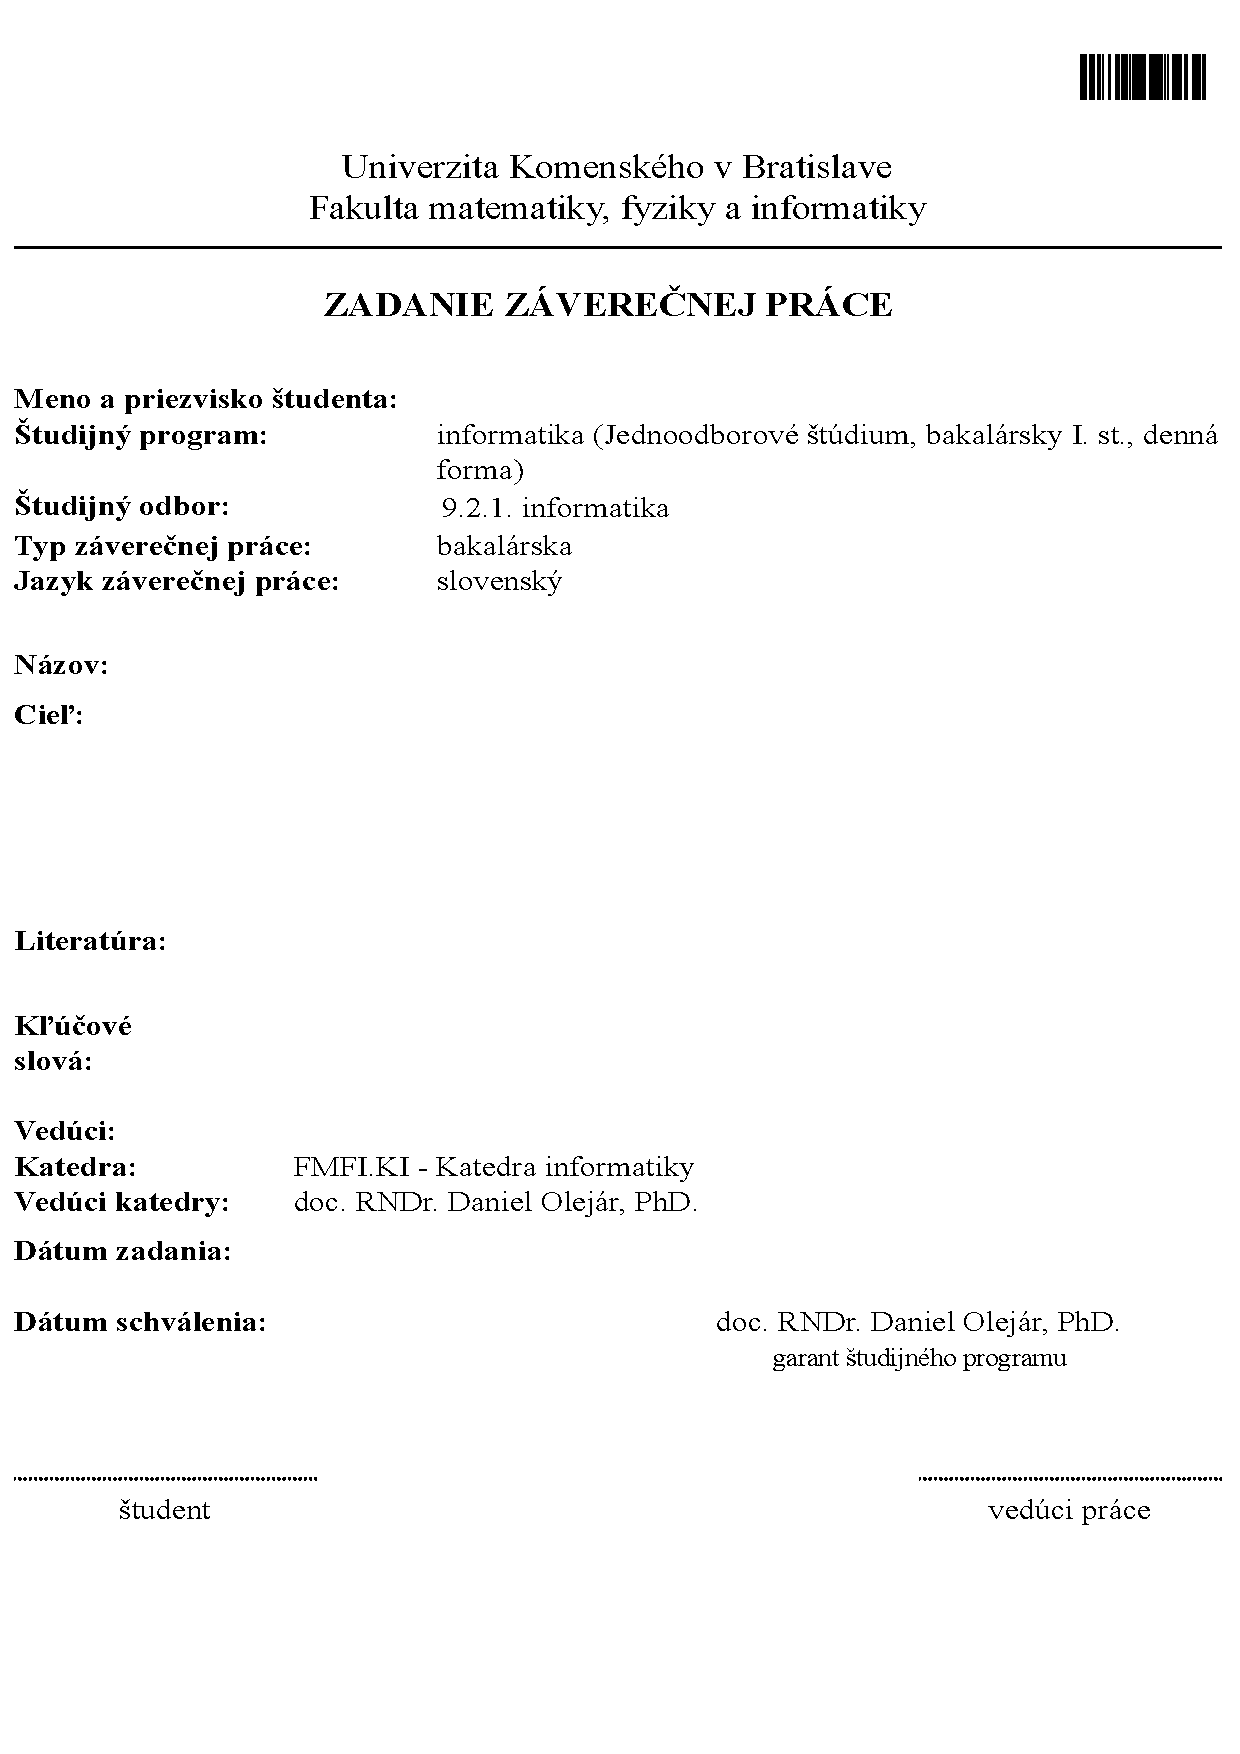
\includegraphics[width=1.4\textwidth]{images/zadanie.pdf}
%\hspace{-1cm}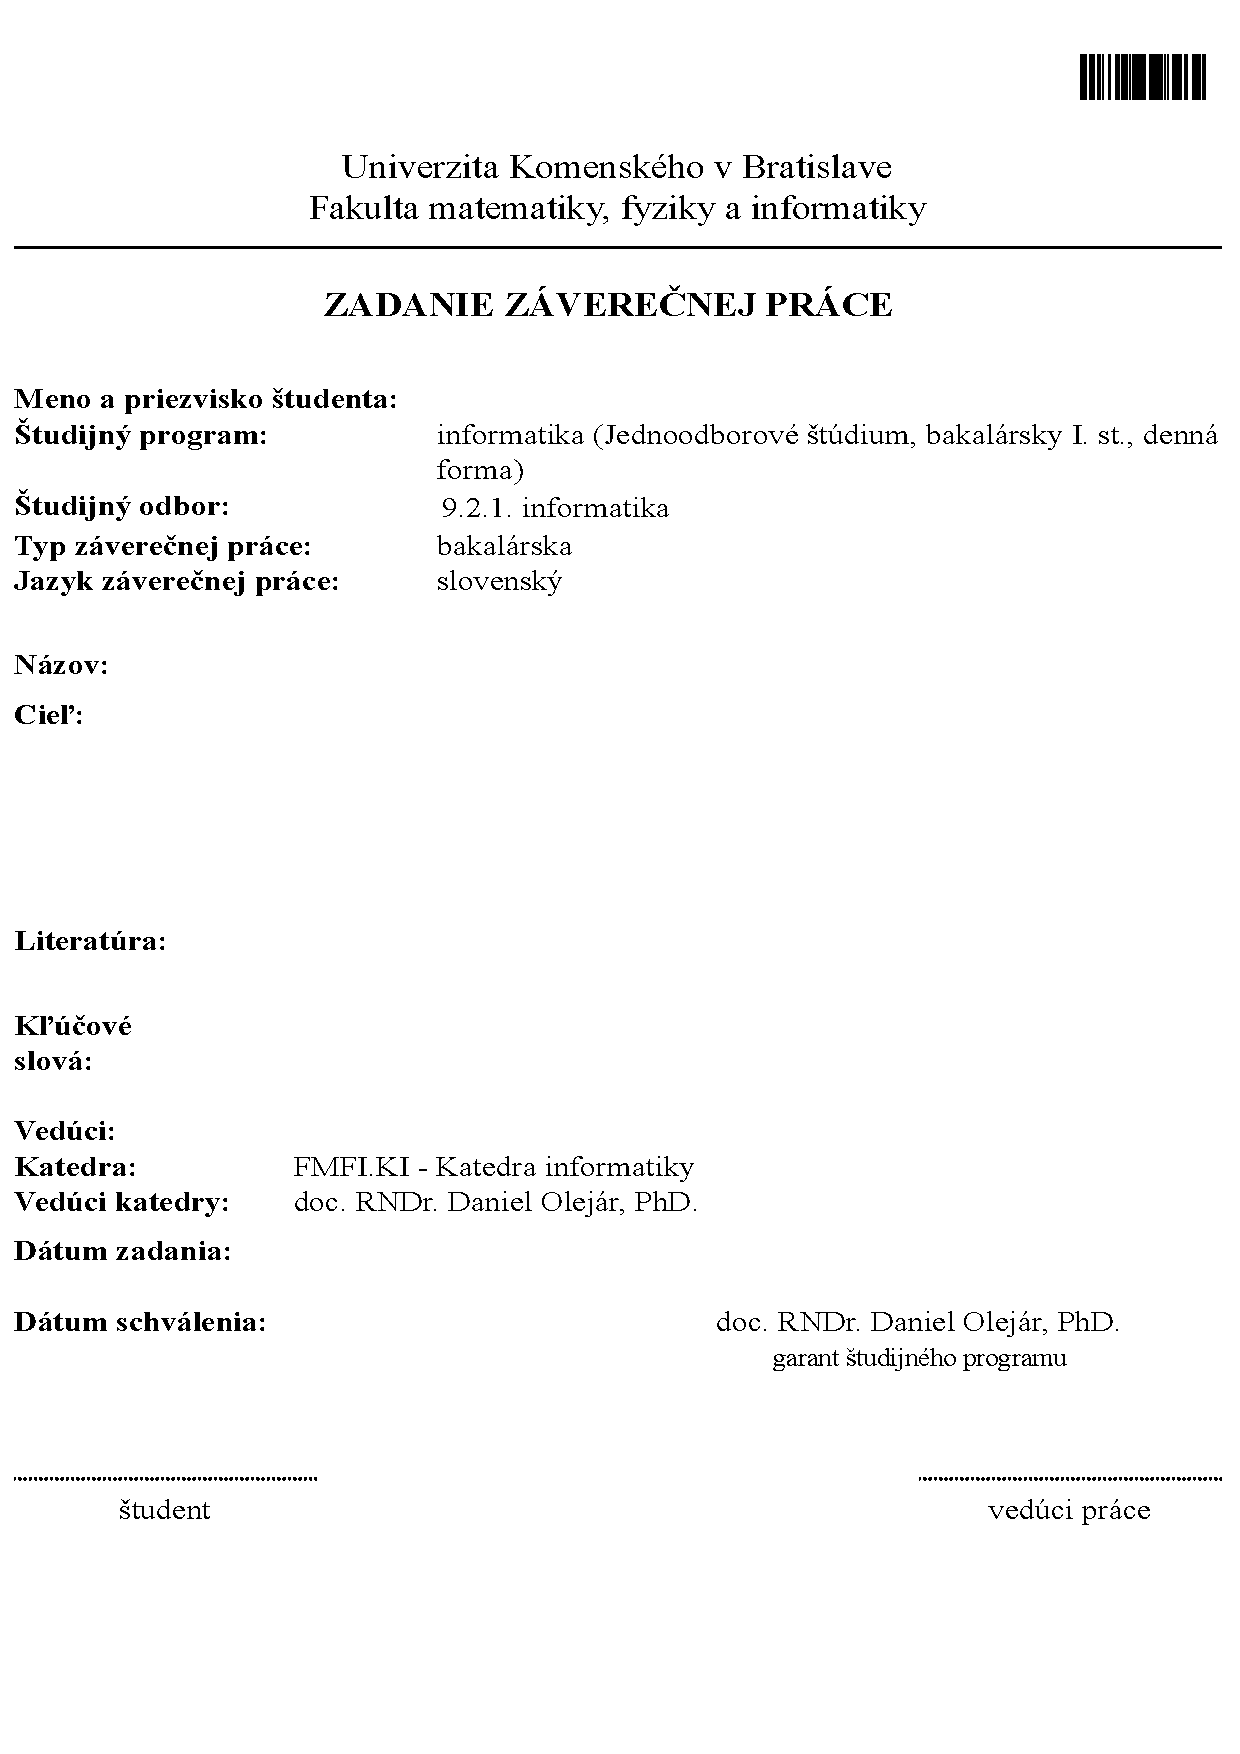
\includegraphics[width=1.2\textwidth]{images/zadanie.pdf}

% --- Koniec zadania

\frontmatter

% -------------------
%   Poďakovanie - nepovinné
% -------------------
\newpage 
\thispagestyle{empty}

\vfill
\huge{Poďakovanie}
%{\bf Poďakovanie:}
\normalsize
\newline

Chcel by som sa poďakovať RNDr. Jaroslavovi Janáčkovi PhD. za odbornú pomoc v oblasti počítačových sietí a za usmernenie pri tvorbe práce.
Ďalej by som sa rád poďakoval všetkým ľuďom a inštitúciam, ktoré mi dovolili použiť ich infraštruktúru a servre na nasadenie honeypot-ov a za to, že som tieto dáta mohol použiť v analytickej a testovacej časti bakalársnej práce.
Tiež by som sa chcel poďakovať svojej rodine a priateľke, ktorí ma podporovali počas celého štúdia.

% --- Koniec poďakovania

% -------------------
%   Abstrankt - Slovensky
% -------------------
\newpage 
\thispagestyle{empty}

\huge{Abstrakt}
\normalsize
\newline

Cieľom bakalárskej práce bolo vytvoriť honeypot na zber prihlasovacích údajov v bežne používaných službách.
V prvej kapitole popisujeme pojem honeypot, jeho kategorizáciu a vysvetľujeme najčastejšie používanú sieťovú architekúru pri práci s honeypot-mi.
Ďalej uvádzame popis všetkých technológií použitých pri tvorbe honeypot-u a jeho implementačné detaily.
Taktiež navrhujeme rôzne postupy, ktorých uplatnením by mohlo dôjsť ku skvalitneniu nazberaných dát a k zvýšeniu ich počtu.
Následne analyzujeme dáta nazberané naším honeypot-om.
Uvádzame štatistiky a rôzne výsledky vyplývajúce z nazberaných údajov.
V zá\-ve\-reč\-nej časti práce prezentujeme metódu, ktorou sme overovali, či existujúci informačný systém nie je zraniteľný na slovníkový útok nami zozberanými heslami.
Prácou sme potvrdili, že klásť dôraz na informačnú bezpečnosť patrí k neodmysliteľným faktorom v súčasnom svete.
\\
\\
{\bf Kľúčové slová:} honeypot, slovníkový útok, PAM, ELK stack, \mbox{oclHashcat}
% --- Koniec Abstrakt - Slovensky


% -------------------
% --- Abstrakt - Anglicky 
% -------------------
\newpage 
\thispagestyle{empty}

\huge{Abstract}
\normalsize
\newline

The aim of the bachelors thesis was to create a honeypot to gather login data from commonly used services.
In the first chapter, we describe the term honeypot, its categorisation and explain the network architecture that is most commonly used when working with honeypots.
Next we present descriptions of all technologies used in creation of honeypot and details of its implementation.
We also design different approaches that improve the quality and quantity of the gathered data.
Afterwards we analyse the data gathered by the honeypot.
We present different statistics and results, which stem from the gathered data.
In the final part of the thesis, we present the method that was used to verify whether the existing information system is vulnerable to dictonary attack using gathered password.
The thesis confirmed that focusing on information security is one of the most importnant concerns in this day and age.
\\
\\
{\bf Keywords:} honeypot, dictionary attack, PAM, ELK stack, oclHashcat

% --- Koniec Abstrakt - Anglicky

% -------------------
% --- Predhovor ?????
% -------------------
%\newpage 
%\thispagestyle{empty}
%
%\huge{Predhovor}
%\normalsize
%\newline
%Predhovor je všeobecná informácia o práci, obsahuje hlavnú charakteristiku práce 
%a okolnosti jej vzniku. Autor zdôvodní výber témy, stručne informuje o cieľoch 
%a význame práce, spomenie domáci a zahraničný kontext, komu je práca určená, 
%použité metódy, stav poznania; autor stručne charakterizuje svoj prístup a svoje 
%hľadisko. 
%
% --- Koniec Predhovor


% -------------------
% --- Obsah
% -------------------

\newpage 
\tableofcontents

% ---  Koniec Obsahu

% -------------------
% --- Zoznamy tabuliek, obrázkov
% -------------------

%\newpage 

%\listoffigures

% ---  Koniec Zoznamov

\mainmatter

\chapter*{Úvod}
\addcontentsline{toc}{chapter}{Úvod}

V ostatných rokoch sa v oblasti informačných technológií začína klásť väčší dôraz na bezpečnosť.
Všetci ľudia, všetky štátne inštitúcie aj podnikateľské subjekty majú záujem o čo najvyššiu ochranu svojich dát, ktoré sú často extrémne citlivé a podľa zákona je potrebné ich chrániť.
Aby sa zamedzilo neautorizovanému prístupu používajú sa rôzne techniky, napríklad dvojfaktorová autentifikácia.
Ale ani tá nemôže zabezpečiť úplnú ochranu.
Preto je dôležitá prevencia pred možnými útokmi.
Ak sa zraniteľnosť odhalí včas, môže sa predísť veľkým problémom.
Cieľom tejto práce je vytvorenie honeypot-u, ktorého úlohou bude zberanie prihlasovacích údajov.
Bude simulovať server s množstvom služieb, a preto bude mať vysoký potenciál na poli zraniteľných ,,obetí''.
Služby bežiace na serveri budú zberať prihlasovacie údaje a dalšie informácie o útočníkoch, ktoré budú neskôr použité na hĺbkovú analýzu a test či nie je existujúci informačný systém zraniteľný na prihlásenie týmito údajmi.

\chapter{Prehľad honeypot-ov}

Úvodom práce by sme spravili prehľad honeypot-ov, na aké typy sa delia a z akých častí pozostávajú.
Pojem honeypot je v informačnej bezpečnosti známy už niekoľko rokov.
Nenájdeme však jednotnú definíciu.
Podľa nášho názoru bol najlepšie vystihnutý v práci honeypot security\cite{hongkong}, ktorý ho definoval nasledovne\footnote{voľný preklad}:

\textit{“Honeypot je klamlivá pasca, navrhnutá tak, aby nalákala útočníka k pokusu ohroziť informačný systém v organizácii.“}

Ďalej pokračoval:

\textit{„Ak je honeypot nasadený správne, môže slúžiť ako systém skorého varovania a pokročilý bezpečnostný nástroj, ktorým sa minimalizujú riziká útokov smerujúcich na IT systémy a siete.“}

Podľa techopedie\cite{technopedia} sa honeypot dá definovať nasledovne\footnote{opäť volný preklad}:

\textit{“Honeypot je provokujúci počítačový systém učený na odchyt útočníkov alebo sledovanie netradičných či nových hekovacích metód.“}

Nech si zoberieme akúkoľvek definíciu, vždy ide o systém, ktorého účelom je zlepšenie sieťovej bezpečnosti sledovaním používaných útočných metód.

\section{Delenia honeypot-ov}

Honeypot-y sa delia do rôznych kategórií, ktoré neskôr rozoberieme. Nie vždy je možné honeypot jednoznačne zaradiť.

\subsection{Podľa typu použitia / typu nasadenia}

\begin{itemize}

\item{Produkčné}

Tento typ honeypot-ov je určený hlavne pre komerčnú sféru.
Jeho účelom je zisťovať, aké útoky sú smerované na firemnú infraštruktúru.
Dobrou a skorou analýzou je možné včas prijať bezpečnostné opatrenia na ochranu pred budúcimi útokmi.
Vo väčšinou simulujú konkrétny operačný systém a službu, ktoré sa vo firme používajú.

\item{Výskumné}

V prípade výskumných honeypot-ov, ide zväčša o reálny operačný systém a služby.
Slúži hlavne na identifikáciu nových typov útokov, ktoré doposiaľ neboli identifikové alebo hlbšie zanalyzované.
Honeypot-y tohto typu nasadzujú univerzity, armáda alebo iné bezpečnostné organizácie.
Výsledky zistení organizácie sú často prezentované pre potreby všeobecného zlepšenia bezpečnosti.

\end{itemize}

\subsection{Podľa interakcie}

\begin{itemize}
\item{Nízko interaktívne}

Už z názvu vyplývajú ich vlastnosti.
Zväčša simulujú určitý operačný systém aj službu, ktorých miera možnosti odpovedať je veľmi nízka.
Výhodou je, že sú ľahko upraviteľné a nasaditeľné.
Tieto honeypot-y sa používajú najmä v produkčnom prostredí. 
\\
\item{Vysoko interaktívne}

Najčastejšie nasadenie týchto honeypot-ov sledujeme vo výskumnom prostredí.
Zväčša ide o reálny operačný systém.
Výhodou je, že pri použití anti-honeypot-ových techník, identifikácia toho, že ide o honeypot a nie o skutočný server je náročnejšia.
Týmto však zvyšuje zraniteľnosť seba samého, avšak často vedie ku skutočnému odhaleniu nových hrozieb.

\end{itemize}

V prípade nášho honeypot-u ide o výskumný, vysoko interaktívny honeypot, i keď v našom prípade neslúži na identifikáciu nových typov útokov, lebo o útokoch slovníkom či hrubou silou\footnote{brute-force} sa už dávno vie.
Jedným z dôvodov vytvorenia honeypot-u je, že v čase tvorby práce sa nám nepodarilo nájsť žiaden honeypot tohto typu na trhu voľne dostupných nástrojov.


\section{Časti honeypot-ov}

Medzi najrozšírenejšie honeypot-ovacie systémy patrí NetFlow od firmy Cisco.
Ide o systém na analýzu sieťovej prevádzky.
Celý monitorovací nástroj je rozdelený na 4 časti.
Uvedenou architektúrou sme sa inšpirovali a využili sme ju aj v prípade nášho honeypot-u a analýzy jeho dát.

Podľa architektúry, kde je NetFlow nasadený, rozdeľujeme jej časti nasledovne: 

\begin{itemize}
\item Exporter
\item Collector
\item Storage
\item Analyzer
\end{itemize}

\begin{figure}[h]
\centering{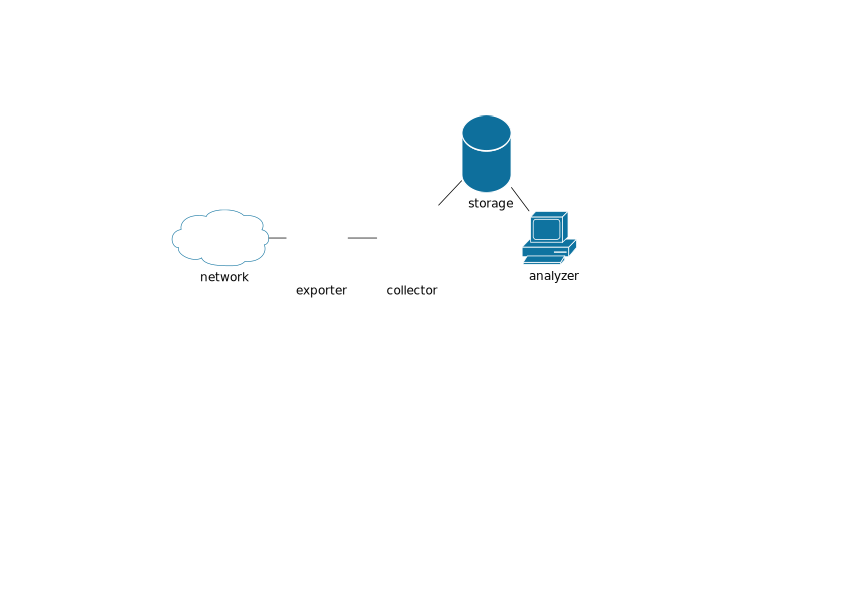
\includegraphics[width=0.8\textwidth]{images/visual}}
\caption{Architektúra}
\end{figure}

\subsection{Exporter}
Najdôležitejšou časťou je exporter. Ten zaznamenáva všetok sieťový prenos a posiela zistené dáta na collector.
Je to najzraniteľnejší prvok v architektúre, nakoľko práve naňho sa útočí.
Exporter je s collectorom zvyčajne prepojený prostredníctvom separátnej siete, aby sa zabezpečila vyššia ochrana získaných dát.

\subsection{Collector}
Úlohou collectora je zberať dáta z exporterov. Z tohto dôvodu je význam hlavne v prípade, že exporterov máme viac.
Samozrejme, dá sa využiť aj v prípade, ak je iba jeden. Collector zberá prijaté dáta a ukladá ich na storage.

\subsection{Storage}
Storage je softvérové úložisko dát.
Najčastejšie ide o skupinu súborov na filesystéme.
Na tento účel sa môže použiť aj databáza ako v našej práci.

\subsection{Analyzer}
Posledným prvkom je analyzér.
Táto časť má za úlohu analyzovať dáta zo storage-u a vracať informácie o zistených výsledkoch.

\chapter{Tvorba honeypot-u}
Účelom honeypot-u, ako aj výsledkom našej práce, je zber prihlasovacích údajov použitých pri útokoch.
Taktiež budeme zberať aj dalšie dáta, ktoré sa nám podarí o útočníkovi zistiť: službu, na ktorú útočil, jeho IP adresu alebo čas, v ktorom uskutočňoval útok.

\section{Použité technológie}

\subsection{PAM}

Pod skratkou PAM sa nachádza Pluggable authentication module.
Je to autentifikačný mechanizmus, ktorý sa využíva vo veľkom množstve Unix-ových systémov.
Ponúka nízkoúrovňové API\footnote{Application programming interface} pre programy, na prevádzanie autentifikácie.
PAM tiež slúži na správu sessions prihlásených užívateľov alebo na zmenu hesla.
My z neho využijeme iba funkciu autentifikácie.
Autentifikačná časť PAM dostane prihlasovacie údaje od služby, ktorá vyžaduje prihlásenie.
Modul sa rozhodne či je prihlásenie možné a podľa potreby vráti vhodnú odpoveď.
Množina odpovedí má okrem štandardných návratových hodnôt ,,úspešne prihlásený'' alebo ,,neúspešne prihlásený'' aj ďalšie odpovede:  ,,nedostatok informácií pre overenie'' alebo ,,zlyhanie modulu'' v prípade, že modul chcel používať prostriedky, ktoré mu neboli pridelené.
Všetky potrebné informácie sú dostupné na stránke projektu\cite{pam} online, ale aj v stiahnuteľnej offline verzii.

Väčšina Unix-ových systémov prináša pri inštalácii veľké množstvo štan\-dard\-ných modulov. Ich umiestnenie je závislé na konkrétnom systéme, ale vo väčšine prípadov sa jedná o \texttt{/lib/security}.

\subsection{MongoDB}

Pre uschovanie údajov z honeypot-u bola použitá NoSQL databáza, konkrétne MongoDB.
Tento typ bol zvolený, pretože sa jedná o dokumentovo-orientovanú databázu\footnote{\texttt{en.wikipedia.org/wiki/Document-oriented\_database}}, čo je výhodné pre účely našej práce.
Hlavným benefitom je jednoduché rozšírenie o ďalšie položky bez potreby zásahu do existujúcej databázy.
Tento prípad môže nastať, ak by sa API autentifikačnej PAM knižnice rozšírilo o ďalšie parametre a niekto by mal potrebu toto rozšírenie zakomponovať aj do implementácie nášho PAM.
Ďalším z plusov je rýchle prehľadávanie.
Okrem už spomenutých vlastností tejto databázy bolo pre nás obohacujúce získavať skúsenosti pri práci s týmto typom databázy.
Databázový server je pre bezpečnosť a možnosť centralizácie (v prípade použitia viacerých honeypot-v) spustený na samostatnom serveri.
PAM sa naň pripája prostredníctvom databázového API.



\subsection{Architektúra}

Honeypot bežal na operačnom systéme Linux, konkrétne na distribúcii Debian.
Aby bolo možné skompilovanie modulu a používanie API funkcií, bolo potrebné nainštalovanie niekoľkých balíčkov:
\begin{itemize}
\item libpam0g
\item libpam0g-dev
\item libmongo-client-dev
\end{itemize}
  
Kompilovanie bolo zjednodušené použitím Makefile-u, ktorý je prílohou našej práce.
Preto bolo postačujúce zadať iba:

\begin{lstlisting}[style=customBash]
make
make install
\end{lstlisting}

Tým sa modul skompiloval a umiestnil so správnymi právami do a\-dre\-sá\-ra \texttt{/lib/security}.
Aby PAM systém vedel, že má používať náš modul, bolo potrebné v súbore \texttt{/etc/pam.d/common-auth} odstrániť všetky riadky a nahradiť ich riadkom:
\begin{lstlisting}[style=customBash]
auth requisite pam_bcpot.so
\end{lstlisting}

Od tohto momentu všetky systémy, ktoré vedia používať PAM a cielene si nezmenili \texttt{auth} pravidlá v \texttt{/etc/pam.d/}, budú využívať na autentifikáciu náš modul.

\subsection{Služby}

Na zber dát bolo použitých niekoľko štandardných služieb, ktorým sa budeme venovať v práci neskôr.
Všetky služby podporujú komunikáciu s PAM kniž\-ni\-cou cez API.

Mali sme záujem zaradiť aj službu SAMBA, ktorá je potrebná na využívanie protokolu smb.
Ten umožňuje zdieľanie prostriedkov, ako prístup k súborovému systému alebo zdieľanie tlačiarní.
Protokol je vo veľkom množstve používaný operačným systémom Microsoft Windows.
Nakoľko je tento operačný systém vo svete veľmi rozšírený, dalo sa očakávať, že bude najväčšie množstvo útokov práve na túto službu. 

Počas nasadzovania a testovania PAM sme však zistili, že samba nepodporuje PAM, a preto sme ju museli z nášho návrhu odstrániť.
V protokole sa totiž neodosiela heslo v plaintext\footnote{čistý text, ktorý neprešiel procesom hašovania}-ovej podobe, ako väčšina protokolov, ale hašuje sa na klientskej strane, a preto ho nie je možné na serveri prečítať.

Uvedená vlastnosť nebola v protokole vždy.
Staršia verzia SAMBA podporovala aj posielanie hesla v plaintext-ovej podobe.
Službu SAMBA je možné zapnúť aj v móde kompatibilnom so spomínanou verziou, avšak to by mohlo byť pre útočníkov podozrivé\footnote{v súčastnosti sa táto možnosť nepoužíva}, a preto bolo lepšie túto službu ignorovať.

Uvádzame zoznam služieb, ktoré boli nasadené na honeypot-e v poradí podľa čísel portov, na ktorých počúvajú.

\subsubsection{FTP server}
Pre tieto účely bol nainštalovaný FTP server odporúčaný distribútorom operačného systému konkrétne vsftpd. Port tejto služby je 21. Pre správnu komunikáciu a bezpečnostnú politiku boli potrebné tieto nastavenia:

\begin{lstlisting}[style=customBash]
listen=YES
anonymous_enable=NO
local_enable=YES
dirmessage_enable=YES
use_localtime=YES
xferlog_enable=YES
connect_from_port_20=YES
secure_chroot_dir=/var/run/vsftpd/empty
pam_service_name=vsftpd
rsa_cert_file=/etc/ssl/private/vsftpd.pem
\end{lstlisting}

\subsubsection{SSH server}
Ako server pre SSH(port 22) bol použitý openssh-server s nasledovnými nastaveniami:

\begin{lstlisting}[style=customBash]
Port 22
Protocol 2
HostKey /etc/ssh/ssh_host_rsa_key
HostKey /etc/ssh/ssh_host_dsa_key
HostKey /etc/ssh/ssh_host_ecdsa_key
UsePrivilegeSeparation yes
KeyRegenerationInterval 3600
ServerKeyBits 768
SyslogFacility AUTH
LogLevel INFO
LoginGraceTime 120
PermitRootLogin yes
StrictModes yes
RSAAuthentication yes
PubkeyAuthentication yes
IgnoreRhosts yes
RhostsRSAAuthentication no
HostbasedAuthentication no
PermitEmptyPasswords no
ChallengeResponseAuthentication no
X11Forwarding yes
X11DisplayOffset 10
PrintMotd no
PrintLastLog yes
TCPKeepAlive yes
AcceptEnv LANG LC_*
Subsystem sftp /usr/lib/openssh/sftp-server
UsePAM yes
\end{lstlisting}

\subsubsection{SMTP server}
Ako mailový server, určený na prijímanie pošty bol zvolený Postfix. Port bol znova štandardný a to s číslom 25. Pravidlá uplatnené v /etc/postfix/main.cf boli nasledovné:

\begin{lstlisting}[style=customBash]
smtpd_banner = $myhostname ESMTP $mail_name (Debian/GNU)
biff = no
append_dot_mydomain = no
readme_directory = no
smtpd_tls_cert_file = /etc/ssl/certs/postfix.pem
smtpd_tls_key_file = /etc/ssl/private/postfix.pem
smtpd_use_tls=yes
smtpd_tls_session_cache_database = btree:${data_directory}/smtpd_scache
smtp_tls_session_cache_database = btree:${data_directory}/smtp_scache
myhostname = atlantis
alias_maps = hash:/etc/aliases
alias_database = hash:/etc/aliases
mydestination = atlantis, localhost.localdomain, localhost
relayhost = 
mynetworks = 127.0.0.0/8 [::ffff:127.0.0.0]/104 [::1]/128
mailbox_command = procmail -a "$EXTENSION"
mailbox_size_limit = 0
recipient_delimiter = +
inet_interfaces = all
smtpd_sasl_auth_enable = yes
smtpd_sasl_security_options = noanonymous
smtpd_client_restrictions = permit_sasl_authenticated
broken_sasl_auth_clients = yes
smtpd_recipient_restrictions = permit_sasl_authenticated, permit_mynetworks, reject_unauth_destination
smtpd_sasl_local_domain = $myhostname
\end{lstlisting}

\subsubsection{Web server}
Na honeypot bol nasadený webový server Apache, počúvajúci na štandardnom porte 80.
Server ponúka na svojom prednastavenom virtualhost-e stránku vyžadujúcu na prístup HTTP Basic autentifikáciu\footnote{\texttt{RFC1945} a \texttt{RFC2617}}, ktorá sa overuje cez PAM.
Taktiež bolo potrebné nainštalovanie modulu \texttt{libapache2-mod-}\\\texttt{-auth-pam}. Nastavenie virtualhost-u teda vyzerá nasledovne:

\begin{lstlisting}[style=customBash]
<VirtualHost *:80>
	ServerAdmin webmaster@localhost
	DocumentRoot /var/www
	<Directory />
		Options FollowSymLinks
		AllowOverride None
	</Directory>
	<Directory /var/www/>
		Options Indexes FollowSymLinks MultiViews
		AllowOverride None
		Order allow,deny
		allow from all
		AuthType Basic
		AuthName "Master Server"
		AuthPAM_Enabled On
		AuthBasicAuthoritative off 
		Require group valid-user
	</Directory>
	ErrorLog ${APACHE_LOG_DIR}/error.log
	LogLevel warn
	CustomLog ${APACHE_LOG_DIR}/access.log combined
</VirtualHost>
\end{lstlisting}

\subsubsection{IMAP(S) a POP3(S) server}
Na čítanie mailov bol zvolený Courier s jeho rozšíreniami.
Pre služby IMAP a POP3 boli zvolené ich štandardné porty 143 a 110. Pre IMAPS a POP3S zase 993 a 995.
Predvolená inštalácia servera bola pre naše potreby vhodná. Museli sme upraviť iba nasledovné nastavenia:

\begin{lstlisting}[style=customBash]
authmodulelist="authpam"
authmodulelistorig="authpam"
\end{lstlisting}

\section{Implementácia modulu}

Skutočnosť, že honeypot mal heslá iba zberať neumožňovala žiadne korektné prihlásenie.
Týmto spôsobom sme chceli donútiť útočníka použiť čo najväčšie množstvo hesiel.
Modul získal požadované dáta a bez akéhokoľvek overovania hesla vyhlásil prihlásenie za neúspešné z dôvodu zadania neplatného  \texttt{AUTHTOK}\footnote{v PAM je takto nazývané zlé heslo}.

Keďže PAM aj MongoDB využívajú prehľadné API, celková im\-ple\-men\-tá\-cia modulu nepresiahla 100 riadkov.

Úvodom programu sú direktívy, ktoré pripájajú potrebné knižnice k nášmu modulu.
Ďalej sa nachádza klauzula:
\begin{lstlisting}[style=customC]
#define PAM_S_AUTH
\end{lstlisting}

Vďaka nej celé PAM vie, že náš systém implementuje funkcie,
\begin{lstlisting}[style=customC]
pam_sm_authenticate
pam_sm_setcred
\end{lstlisting}
ktoré sa musia podľa špecifikácie nachádzať v module v prípade, že chceme vykonávať autentifikáciu.

V úvode \texttt{pam\_sm\_authenticate} je volanie funkcie, ktorá slúži na nadviazanie spojenia s collectorom.
Na tomto mieste je preto, aby sme v prípade zlyhania nerobili žiadne zbytočné kroky naviac, napríklad zisťovanie hesla.
Na tento účel bol použitý príkaz:
\begin{lstlisting}[style=customC]
conn = mongo_sync_connect( "collector", 27017, FALSE );
\end{lstlisting}

%Funkcia \texttt{mongo\_sync\_connect} má 3 parametre.
%Meno alebo IP adresa servera, port, na ktorom počúva.
Server sme pomenovali ,,collector''.
Pre správne preloženie mena na IP adresu by bolo možné vytvoriť DNS záznam.
V našom prípade sme uprednostnili jednoduchšiu voľbu a to vpísanie do súboru \texttt{/etc/hosts}.
Čislo portu sme zvolili na štandardnú hodnotu 27017.

V ďalšom kroku sme vytvorili BSON objekt prostredníctvom \texttt{bson\_new()}.
Túto štruktúru využíva MongoDB na zápis údajov.

Nasledovalo vyžiadanie si hesla prostredníctvom callback-u 
\begin{lstlisting}[style=customC]
pam_get_authtok( pamh, PAM_AUTHTOK, (const char*)
    &password, NULL );
\end{lstlisting}

Bez tohto kroku by nám heslo nebolo doručené, lebo niektoré systémy umožňujú prihlásenie bez zadania hesla.
Ďalej sme si vypýtali všetky údaje, ktoré boli podľa aktuálnej implementácie PAM\cite{pam} dostupné.
Veľká časť z nich sa bežne nevyužíva, ale vzhľadom na možnosti použiť tento modul s ľubovoľnou službou boli použité všetky.
V prípade, že dáta boli ne\texttt{NULL}ové, uložili sme ich do BSONu.

Pridali sme aj hostname, aby sme v prípade viacerých honeypot-ov vedeli, z ktorého nám informácia prišla.

BSON sme nakoniec uzavreli, poslali sme ho na \texttt{collector} a spojenie sme uzavreli.

Ukončenie funkcie bolo zavolané s parametrom \texttt{PAM\_AUTHERR}, ktorý, ako už bolo spomenuté, oznamuje zadanie zlého heslo.

Na konci celého modulu je ešte funkcia \texttt{pam\_sm\_setcred}, ktorá je povinná v prípade tvorby autentifikačného modulu.
My ju však nevyužívame, a preto má automaticky návratovú hodnotu \texttt{PAM\_SUCCESS}.

Ponúka sa aj zmena implementácie, nakoľko časté otváranie spojenia s databázou, ktorá je dokonca na inom serveri, môže byť zdĺhavé.
Môže tým byť znížená efektivita, a teda aj potenciál získania väčšieho množstva dát.
Na druhej strane, systém by možno odpovedal prirýchlo, čo by sa útočníkovi mohlo zdať podozrivé.

\section{Možnosti zlepšenia}

Na zvýšenie atraktivity honeypot-u, by bolo možné vykonať niekoľko zlepšení.

V prvom rade by bolo vhodné vytvoriť reálne vyzerajúci DNS záznam, čím by server pôsobil dôveryhodnejšie.

Ďalšou možnosťou je zverejnenie IP adresy alebo už spomenutého DNS záznamu na internete.
Za najvhodnejšiu formu však môžeme považovať zverejnenie adresy resp. záznamu na webovom fóre alebo inej stránke.
Potenciálni útočníci sa tak o honeypot-e dozvedia.

Faktorom spojeným s DNS je vytvorenie SPF záznamu\footnote{Sender policy framework - \texttt{RFC7208}}, ktorý by pridal na dôveryhodnosti mailového serveru.

Posledným rozšírením môže byť vyhlasenie, že sa na honeypot-e nachádza a\-trak\-tí\-vny obsah.
Tieto informácie by mohli byťuverejnené opäť na fórach alebo priamo na webovom serveri honeypot-u.
Priestor na stránke by sa tým pádom rozdelil na utajený\footnote{s potrebou prihlásenia, ktoré by bolo naviazané na PAM} a na verejný\footnote{s prehlásením o obsahu, ktorý sa nachádza v utajenej časti}.
Obsah by mohli byť tvorený filmami, ktorých premiéra sa práve chystá alebo je tesne po premiére, utajovanými informáciami či citlivými informáciami, napríklad osobné údaje podliehajúce ochrane na základe zákona.


\chapter{Analýza získaných údajov}

V tejto časti práce sa budeme venovať analýze útokov.
Útok je v krátkom výkladovom slovníku termínov informačnej bezpečnosti definovaný nasledovne\cite{ksib}:

\textit{Cieľavedomý pokus o využitie nejakej zraniteľnosti systému/aktíva za účelom získania neoprávnených privilégií alebo poškodenia/zneužitia daného aktíva, alebo niektorého z iných aktív systému/organizácie.}

V našom prípade by sme za zraniteľnosť mohli považovať slabé heslo do informačného systému a za účel, v prvom rade, získanie neoprávnených privilégií.

Prejdime však k samotným dátam.
Ich zber bol prevádzaný na jednom mieste, išlo o virtuálny stroj.
Honeypot sa nachádzal na Fakulte matematicky, fyziky a informatiky Univerzity Komenského v Bratislave.
Bol nasadený vďaka spolupráci s Katedrou informatiky.

Dáta boli zberané 63 dní. Za tento čas sa podarilo nazberať 1~089~604 záznamov.
Je dôležité spomenúť, že útočníci našli server skenovaním sieťového rozsahu. Jeho IP adresa alebo iná informácia o jeho existencii nebola nikde zverejnená.

\section{ELK Stack}
Na analýzu dát bol použitý mechanizmus nazývaný ELK Stack.
Ide o spojenie troch open-source-ových nástrojov. 
\subsection{Logstash}
Programovacím jazykom je Java a je určený na parsovanie rôznych formátov, ďalšiu úpravu a ukladanie do rôznych formátov či databáz. Práca, ktorú robí logstash s každým záznamom je rozdelená do troch fáz:
\begin{itemize}
\item Input
\item Filter
\item Output
\end{itemize}

V časti input sa popisuje, z čoho má čerpať dáta. Najčastejšie ide o súbor, ktorý je v špecifickom formáte alebo je možné nastaviť ho do režimu, kedy počúva na vybranom TCP alebo UDP porte a spracúva všetky tieto dáta. Dáta pre spracovanie logstashom sme najprv exportovali z databázy collectora nasledovným príkazom \texttt{mongoexport --db local --collection bcData > export.json}, ktorého výstupom bol súbor vo formáte JSON\footnote{JavaScript Object Notation - ľudsky čitateľný objektový formát, ktorý je definovaný v \texttt{RFC7159}}.
Následne sme ich načítali logstashom, jeho pravidlom file.

Vo fáze filter logstash mení, maže či dopĺňa dáta na základe určených pravidiel.
V našom prípade sme preložili DNS\footnote{http://logstash.net/docs/1.4.2/filters/dns} záznam počítača na IP adresu, ktorý na nás útočil, pričom pôvodný názov sme si tiež odložili\footnote{PAM totiž ukladal popis útočníka v tvare jeho DNS záznamu alebo IP adresy, na základe toho akú informáciu mu posunula služba, na ktorú bolo útočené(ak je mu informácia vôbec poskytnutá)}.
Použili sme aj mechanizmus GeoIP\footnote{http://logstash.net/docs/1.4.0/filters/geoip}, ktorý dokáže zistiť na základe IP adresy geografickú polohu jej vlastníka.
Nie vždy sa dá táto pozícia určiť presne.
Vo veľkom počte prípadov sa dá identifikovať aspoň štát, z ktorého sa útočilo.
Pridáli sme aj položky, ktoré nám budú pomáhať pri analýze, napríklad dĺzka hesiel alebo zhoda prihlasovacieho mena s heslom.

V záverečnej fáze si môžeme určiť, kam sa spracovaný záznam zapíše.
Najčastejšie sa využíva zápis do súboru alebo do databázy elasticsearch. 
V našom prípade sme použili práve zápis do databázy elastichsearch a tiež zápis do súboru, kde sa zapisujú len heslá\footnote{tento súbor nám bude slúžiť v poslednej fáze práce}.

Celý konfiguračný súbor je uvedený v prílohe.

\subsection{Elasticsearch}
Podobne ako v prípade MongoDB aj v prípade Elasticsearch sa jedná o document-oriented databázový systém.
Je optimalizovaný na in-memory-computing\footnote{výpočty, kde sa preferuje uloženie veľkého množstava dát do operačnej pamäte, aby získavanie dát z diskov bolo vyvolané len v prípade potreby, čím sa znižuje počet I/O operácií, čo vedie k celkovému zrýchleniu} a distribuované rozdelenie dát na viaceré počítače.

V tejto databáze budeme uschovávať dáta počas ich analyzovania, nakoľko chceme využiť potenciál rýchleho vyhľadávania.

\subsection{Kibana}
Kibana je názov GUI\footnote{z angl. grafické užívateľské rozhranie} napísaneho v jazyku JavaScript, ktorý sa vykonáva vo webovom prehliadači.
Na analýzu bola použitá verzia 3 aj verzia 4, lebo každá z nich ponúka rôznu bonusovú funkcionalitu.
Kibana si prostredníctvom HTTP pýta dáta v JSON formáte z elasticseach databázy.

Tento nástroj umožňuje rýchlu vizualizáciu prostredníctvom top tabuliek\footnote{tabuľka, kde sú dáta zoradené vzostupne podľa určitej hodnoty}, grafov rôznych druhov\footnote{koláčové, stĺpcové a iné} či máp.

\section{Vlastnosti dát}
Skôr, ako prejdeme k analýze skutočností, ktoré vyplývajú z nazberaných záznamov, uvedieme si rôzne vlastnosti týchto dát.
Zo zdrojového kódu nášho PAM je možné vidieť, ktoré informácie zasielame do databázy. 
Sú to:
\begin{itemize}
\item \texttt{authtok} (heslo)
\item \texttt{service} (služba)
\item \texttt{user} (užívateľ)
\item \texttt{rhost} (meno vzdialeného hosta)
\item \texttt{user\_prompt} (prompt)
\item \texttt{tty} (terminál)
\item \texttt{ruser} (vzdialený užívateľ)
\item \texttt{oldauthtok} (staré heslo v prípade zmeny)
\item \texttt{fail\_delay}
\item \texttt{xdisplay}
\item \texttt{xauthdata}
\item \texttt{authtok\_type}
\end{itemize}

Pridali sme aj \texttt{hostname} honeypot-u pre prípadné potreby odlíšenia.

Na naše účely nám postačuje poznať prvé štyri informácie.
Žiaľ, nie každá služba umoňuje túto podporu.
Konkrétne služby POP3, IMAP a SMTP neuvázda \texttt{rhost}, takže nie je možné určiť pozíciu útočníka.

Za zmienku určite stojí aj obsah \texttt{rhost}. Malo by ísť o adresu útočníka, avšak je na službe, ako túto položku vyplní.
V prípade WEB a FTP servera, ide o IP adresy, zatial čo u SSH ide o reverzný DNS záznam.
Ak ho nie je možné zistiť, ide tiež o IP adresu.
Nie je vylúčené, že iné služby využívajúce PAM budú túto položku vypĺňať na základe mena, ktorým sa im servre predstavia.
Tento fakt by mohol viesť k zavádzaniu útočníkom a k znehodnoteniu používaných dát.

Z dôvodu, ktorý už bol spomenutý\footnote{SSH vypĺňa \texttt{rhost} reverzným DNS záznamom, ak je zistiteľný}, je pre potreby lokalizovania potrebné urobiť pri pársovaní DNS lookup\footnote{preloženie DNS názvu na IP adresu}, ktorý sa vykoná v logstashi filtrom DNS\footnote{pozri podkapitola Logstash}.
Získame tak IP adresu útočníka, z ktorej bude možné vďaka databáze GeoIP geograficky špecifikovať pôvodcu útoku.

Ďalšia nepríjemná vlastnosť dát spočíva v neschopnosti rozlíšiť od seba služby POP3 od POP3S a tiež IMAP od IMAPS.
Túto nepríjemosť spôsobuje, že ide o jednu a tú istú službu, ktorá používa rovnaké pravidlá v PAM a predstavuje sa zhodne.
Jediným rozdielom je, že pred POP3S a IMAPS je vložená vrstva TLS/SSL.

Okrem iného boli pridané: dĺžka použitého hesla a príznak či sa heslo zhoduje s prihlasovacím menom.

Po spustení analýzy dát sa ukázalo, že niektoré z hesiel sú \\\texttt{\textbackslash b\textbackslash nINCORRECT}.
Počas vývoja a testovania sa takýto prípad neobjavil a podobný stav nebol nikde v dokumentácii popisovaný.
Nebolo možné predpokladať, že položka môže nadobudnúť takúto hodnotu.
Pri dodatočnom testovaní sa ukázalo, že spomínaná situácia nastáva v prípade, keď v službe SSH, útočník zadá meno, ale heslo nie a namiesto toho uzavrie spojenie.
Pri analýzach týkajúcich sa hesiel sme tieto položky ignorovali\footnote{až na jeden prípad, ktorý uvedieme}, nakoľko nemajú žiadnu výpovednú hodnotu.
V ostatných prípadoch sme použili na analýzu aj záznamy s touto vlastnosťou.


\section{Analýza dát}

V nasledujúcej časti sa opíšeme podrobnejšiu analýzu získaných dát.

\subsection{Prihlasovacie mená}

Zoznam 100 najpoužívanejších mien je uvedený v prílohe.
Pre\-vlá\-da\-jú\-cim menom je \texttt{root}, tvorí ho až 96\% všetkých skúšaných mien.
Nájdeme tu aj iné pomenovania pre spávcu systému, napríklad \texttt{admin}, \texttt{sysadmin}, \texttt{webadmin} čí \texttt{administrator} (napísaný správne alebo s chybami).

Sledujeme tiež predvolené prihlasovacie mená do rôznych operačných sys\-té\-mov, služieb, monitorovacích systémov či databových služieb: \texttt{nagios}, \texttt{oracle}, \texttt{zabbix}, \texttt{ubnt}, \texttt{www}, \texttt{git}, \texttt{postgres}, \texttt{apache}, \texttt{tomcat}, \texttt{ftpuser}, \texttt{pi}, \texttt{samba}, \dots

\subsection{Prihlasovacie heslá}

Najpoužívanejšie heslo bolo \texttt{wubao}, čo sa ukázalo, že v angličtine znamená \texttt{false}\footnote{slovensky: falošný, nesprávny, nepravdivý}.
Ak sa pozrieme na zastúpenie spomínaného hesla vzhľadom na krajinu, zväčša sa použiva v čínskych IP adresách a zopárkrát sme ho našli aj v japonských.
Z analýzy útočiacich IP adries je vidieť, že ide o botnet,
% v rovnakej sieti
keďže IP adresy zariadení sú si veľmi podobné a líšia sa až v poslednom čísle.

Prípad druhého najpoužívanejšieho hesla je zhodný s predchádzajúcim prí\-kla\-dom.
Opäť ide o rovnaké IP adresy.
V tomto prípade sa jedná o heslo \texttt{jiamima}, čo v preklade znamenená \texttt{plus heslo}. 

Ďalsie heslá sú prevažne číselné. Často ide o sekvenciu rovnakých čísel alebo o rastúcu či klesajúcu postupnusť.

Objavujú sa tiež heslá odpovedajúce operačným systémom. Poukazuje to na predpoklad útočníkov o menej skúsených užívateloch, ktorí nemenia prednastavené heslá. Druhou možnosťou predpokladu je, že kvoli ľahšiemu zapamätaniu si ich schválne nastavujú na rovnaké meno ako typ systému, aby sa ľahšie pamätali.

\subsection{Dĺžky hesiel}

\begin{figure}[h]
\centering{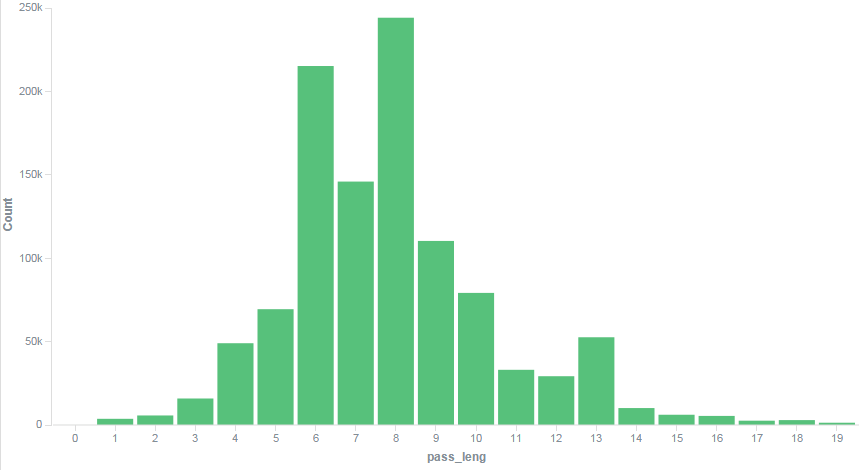
\includegraphics[width=0.8\textwidth]{images/countXpass_leng}}
\caption{Dĺžky hesiel v závislosti od počtu použití v rozsahu 0 až 19 znakov}
\end{figure}

Dĺžka hesiel je ďalší zo skúmaných faktorov.
Na vzorke hesiel do dĺžky 20 znakov sa nám črtá skoro až Gaussovo rozdelenie, pričom navyšší bod je v dĺžke 8.
Možno dedukovať predpoklad útočníkov, že kratšie heslá už užívatelia nepovažujú za dostatočne bezpečné.
Ďalším možným predpokladom je, že užívatelia v heslách používajú slová z domáceho jazyka a majú tendenciu vyberať si slová tejto dĺžky.
Dlhšie heslá si zase nezvyknú vyberať, nakoľko sú náročnejšie na zapamätanie.
Počet hesiel nad spomenujú dĺžku je zanedbateľný.
Zaujalo nás najdlhšie, až 121 znakové heslo:
\texttt{ body \{ font-family:tahoma, verdana, arial, helvetica, sans; \\font-weight:normal; font-size:9pt; background-color:\#eef; \}}.


\subsection{Súvislosť mien a hesiel}

Súvislosti medzi menami a heslami je náročné vyhodnotiť.
Neexistuje konkrétny predpis funkcie, ktorý by presne popisoval vzťah medzi nimi, nakoľko sa tento pojem nedá presne definovať.
Pre tento typ sme zvolili porovnanie zhodou.
Rátali sme, v koľkých prípadoch je meno zhodné heslom.

Na prvom mieste sa nachádzalo meno/heslo \texttt{root}.
V prílohe môžeme vidieť, že ostatné mená/heslá tvoria oproti nemu zanedbateľnú skupinu. 

Z celkového počtu pokusov išlo v 65\% o Čínu.

\subsection{Zastúpenie v rámci služieb}

Pomerové zastúpenie jednotlivých služieb je veľmi špecifické, keďže službe SSH prislúcha až 99.978\% všetkých útokov.
Ostatné služby\footnote{zastúpenie bez SSH zaokruhlené na celé percentá}:

\begin{itemize}
\item WEB 66\%
\item SMTP 15\%
\item POP3 13\%
\item FTP 5\%
\item IMAP 0\%
\end{itemize}

K významnému zastúpeniu SSH mohli prispieť dva faktory.
V prvom rade popularita tejto služby.
Dôvodom je vysoký predpoklad, že ak sa podarí prihlásiť prostredníctvom tejto služby, útočník získa prístup k službám a dátam.
V druhom rade ide o ,,slabú propagáciu'' ostatných služieb verejnosti z pohľadu nášho honeypot-u.
Ná\-po\-moc\-ným prvkom by bolo zakúpenie dôveryhodne vyzerajúcej domény, vytvorenie SPF záznamu či splnením ďalších faktorov, ktoré už boli uvedené v podkapitole ,,Možnosti zlepšenia''.

\subsection{Zdroje útokov}

Mnohé informačné portály tvrdia, že najväčšie množstvo sieťových útokov prichádza z Číny a Ruska.
Z našich štatistík\footnote{boli ovplyvnené tým, že sa zamariavame čisto na útoky spojené so skúšaním hesiel, nemáme žiaden DNS záznam a honeypot bol umiestnený na Slovensku} vyplýva, že v prípade prvého štátu sa táto informácia potvrdila, ale v prípade druhého už nie.
Konkrétne čísla sú uvedené v prílohe, kde je tiež uvedený zoznam 46 krajín, z ktorých prichádzali útoky.
V ostatných 642~786 prípadoch sa nepodarilo na základe IP adresy identifikovať zdrojovú krajinu.
Fakt, že sa jedná o nadpolovičnú väčšinu všetkých záznamov, nami prezentované dáta môžu byť veľmi skreslené.

Dva najviac útočiace štáty, ktoré sa nám podarilo identifikovať, boli Čína a Japonsko, skoro v rovnakom pomere.
Ostatné krajiny boli v výrazne nižšom počte.

Štát, ktorý nás pri analýze zaskočil bol Mjanmar, s pre\-hľa\-dom predbehol veľmoci ako Rusko či Francúzsko.
Pri analýze IP adries sa ukázalo, že išlo skoro v 100\% o jedného útočníka.

Na základe podobných IP adries sme usúdili, že na nás útočili aj botnetové siete.
V prípade jednej sa nepodarilo identifikovať štát, avšak v ostatných prípadoch išlo o japonské a čínske IP adresy.
Pri inej sieti sa ukázalo, že počet hesiel je zhodný alebo išlo o násobky čísla 500.
Výpis použitých hesiel tejto siete ukazuje, že nenachádzame zhodu a heslá jednotlivých útočníkov sú zoradené abecedne.
Toto zistenie indikuje, že ide o botnet so spoločným slovníkom, pričom každý z útočníkov má pridelený rozsah hesiel na skúšanie, resp. sú mu pridelené na požiadanie.

\subsection{Služby vs. prihlasovacie mená}

Pozrieme sa aj to či existuje závislosť medzi prihlasovacími menami a službami.

V prípade SSH, na ktorý smerovalo najväčšie množstvo útokov nie je prekvapivá informácia, že najväčšie množstvo mien bolo \texttt{root}.
Je to spôsobené tým, že ak by útočník prelomil heslo práve tohto užívateľa, podarilo by sa mu ovládať celý systém.
Prelomenie hesla iného užívateľa mu totižto nezaručuje, že by bol neskôr schopný získať privilegovaný prístup, napríklad príkazom \texttt{sudo}

V prípade web servera sa na poprednom mieste ukazujú okrem o\-ča\-ká\-va\-né\-ho root aj heslá admin alebo tomcat\footnote{názov rozšíreného open-source webového servera}.

V ostatných službách útočilo veľmi nízke množstvo útočníkov, čo nám bráni vyslovovať jednoznačné závery.
Jedinou, za zmienku stojacou informáciou, je, že v službe FTP bolo jedenkrát použité prihlasovacie meno \texttt{anonymous}, čo je v tejto službe meno užívateľa používaného na anonymný prístup.

\subsection{Prihlasovacie mená a heslá vs. poloha zdroja}

Ako už bolo spomenuté, pri útokoch z Japonska a Číny boli často použité heslá \texttt{wubao} a \texttt{jiamima}. Iné špecifikum pre tieto štáty nebolo nájdené.

Útočník zo Španielska bol iba jeden\footnote{bolo ich viac, ale aktivita ostatných bola tak nízka, že ju môžeme zanedbať} a jeho popis je uvedený neskôr v kategórii zaujímavých útokov.

Pri útokoch z USA sa nepodarilo nájsť žiadne špecifikum. Tento fakt je s vysokou pravdepodobnosťou ovplyvnený tým, že veľké množstvo terminológie v oblasti IT je v angličtine, a preto použitie slov či mien z tohto jazyka nepovažujeme za zváštne, nakoľko sa používajú aj pri útokoch z iných štátov.

V útokoch z ostatných štátov sa tiež nepodarilo nájsť žiaden signifikantný narást mien či hesiel v dotyčnom jazyku.

\subsection{Časy útokov a súvislosť so zdrojmi útokov}

Časy útokov z Číny boli rovnomerne distribuované počas celého dňa. Tento fakt môže poukazovať na to, že heslá sú skúšané prevažne zo serverov, resp. iných strojov, ktoré nemajú tendenciu vypínať sa, napríklad kvôli určitej pracovnej dobe alebo potrebe prenosu.

Opačný prípad predstavujú útoky z Japonska, kde môžeme sledovať najväčší nárast útokov medzi 4:00 a 6:00 SEČ, čo v Japonsku zodpovedá času medzi 12:00 a 14:00.
Môžeme dá usúdiť, že aktivita sa zvýšuje počas obeda, kedy pravdepodobne veľké množstvo ľudí nevyužíva svoje pracovné stanice, čo je vhodný čas na preniknutie do stroja.

V prípade dát zo Španielska je možné vidieť, že najvýznamnejší útok bol jeden, bol kontinuálny a celý sa udial v poobedných hodinách.

Na druhú stranu, útoky z USA sa diali v tamojších dopoludňajších hodinách.

Iné špecifiká neboli zaznamenané.

\subsection{Iné zaujímavé zistenia}

V predchádzajúcej kapitole sme spomenuli, že časť hesiel bola identická s reťazcom \texttt{\textbackslash b\textbackslash nINCORRECT}.
Po vizualizácii len týchto hesiel sa ukázalo, že boli rovnomerne distribuované počas celého zberu dáť, až na jeden výkyv, ktorému 24941 z 39297 pokusov.
Všetky tieto pokusy vychádzali z jednej Španielskej IP adresy.
Útočník mal atypickú stratégiu, ktorú sme nikde inde nepozorovali.
Najprv skúsil 12 prihlasovacích mien používaných štandardnými unixovskými systémami a heslami, ktoré boli totožné s ich menami.
Nás\-led\-ne spustil vlnu slovníkového skúšania prihlasovacích mien, pričom k žiad\-ne\-mu nezadal heslo.
Mená skúšal v abecednom poradí.
Predpokladáme, že útočník sa pokúšal zistiť, či v systéme neexistuje užívateľ, ktorý by sa mohol prihlásiť bez hesla.

Za zmienku stojí aj jediný útok zo Slovenska.
Išlo zhodou okolností o útočníka z Fakulty matematiky, fyziky a informatiky Univerzity Komenského.
DNS záznam nám naznačuje, že išlo o počítač patriaci organizátorom KSP\footnote{Korešpondenčný seminár z programovania \texttt{http://www.ksp.sk/}}.
Na útok bol použitý len jeden pokus a to s prihlasovacím menom \texttt{gate}.
Heslo však nebolo zadané a komunikácia bola ukončená.

\chapter{Test na dátach}

Poslednou časťou práce je otestovanie dát, ktoré sme nazberali. Zisťovali sme nakoľko sa zhodujú prihlasovacie heslá použité pri útokoch a na existujúcich IS\footnote{informačný systém}.

Výsledky tejto časti nie je možné z bezpečnostných dôvodov zverejniť. K~dispozícií sú iba nástroje, ktorými sa testy vykonávali a krátka štatistika ús\-peš\-nos\-ti prelomenia.

\section{oclHashcat}

Tento nástroj, ktorého autorom je Jens ,,atom'' Steube, slúži na hľadanie pôvodného znakového reťazca z existujúcej hašovacej hodnoty.
Pri zisťovaní sa nevyužívajú žiadne známe zraniteľnosti hašovacích funkcií.
Nástroj jednoducho skúša mož\-nos\-ti podľa zvolenej konfigurácie.
Medzi najpoužívanejšie patrí brute-force, ale je tiež schopný použiť vopred zadaný slovník či ich vzájomnú kombináciu.
Predchodca tohto nástroja \texttt{hashcat} vedel rátať haše len prostredníctvom procesora.
Rozšírená verzia(\texttt{oclHashcat}) vie rátať paralelne na viacerých grafických kartách, čím sa podstatne zvyšuje účinnosť.
OclHashcat ma implementované scenáre hašovania pre rôzne systémy.
Od štandardného hašovania MD5 a sha1, cez použitie salt-u až po viacnásobné využitie hašovacej funkcie na rovnaký reťazec.
Sú k dispozícii kompiláty pre rôzne operačné systémy.
V našom prípade sme použili verziu pre Linux.
Veľké množstvo informácií o programe je možné nájsť na stránke vývojarov\cite{oclhashcat} alebo na ich fóre\footnote{http://hashcat.net/forum/}.
Vývoj oboch nástrojov (\texttt{hashcat} aj \texttt{oclHashcat}) sa posúva stále dopredu a každá nová verzia je závislá na najaktuálnejších ovládačoch grafickej karty (v prípade \texttt{oclHashcat})

Ako už bolo povedané, oclHashcat aj Hashcat slúžia na hľadanie znakového reťazca z jeho hašovanej hodnoty.
Program má k dispozícii rôzne druhy útokov.
My sa zameriame na jeden, konktrétne slovníkový útok.
V prvom rade bolo potrebné pripraviť množinu hesiel.
Tú sme získali pri parsovaní logstashom.
V tomto momente je to zoznam všetkých hesiel, pričom sa v ňom nachádza veľké množstvo duplikátov.
Pre upratanie a zredukovanie sme použili štadnardné unixovské nástroje sort a uniq:

\texttt{cat password\_list.csv | sort | uniq > passwords}

Odstránením duplikátov sa z našich pôvodných 1~089~604 hesiel stalo 312~010, čo zodpovedá približne 29 \%.

Distribúcia Kali obsahuje Hashcat aj oclHashcat vo svojich repozitároch.
Ostatní záujemci sú nútení stiahnuť si program zo stránky autora. 
V~prípade oclHashcat-u je možné zvoliť si správnu verziu, keďže sú závislé od výrobcu grafickej karty. 
Software si tiež overuje, aký driver grafickej karty je nainštalovaný. 
V prípade zistenia, že driver je staršieho dáta, odmietne rátať.
Algoritmy, ktorými počíta sa často spoliehajú na širšiu sadu funkcií, ktorá prichádza s inštaláciou nového driveru.

Hashcat aj oclHashcat dokážu rozoznať o aký typ hašovanej hodnoty sa jedná, avšak niekedy je možné, že reťazec môže byť výsledkom rôznych hašovacích funkcií. 
Pre tieto prípady je lepšie poznať presný typ hašovacej hodnoty, ktorý chceme prelomiť a explicitne ho definujeme s pomocou prepínača „-m“.

Rátanie spustíme nasledovným príkazom:
\texttt{oclHashcat64.bin -m 1800 hashFile --username passwords --outfile=cracked\_passwords}

Proces počítania je možné priebežne sledovať a v prípade potreby pozastaviť alebo uplne zrušiť.

V prípade prelomenia hesla sa dvojica v zložení hašovaná hodnota a prelomené heslo objavia v nami definovanom súbore cracked\_password.

\section{Výsledky testovania}

Hašované hodnoty hesiel boli tri typy: descrypt, MD5 a SHA256.
Dáta sme prevzali z databázy a boli anonymizované.
Z celkového počtu 2550 hašov sa podarilo slovníkovým útokom prelomiť 34 hesiel.

\chapter*{Záver}
\addcontentsline{toc}{chapter}{Záver}

Informačná bezpečnosť je oblasť, na ktorú sa v súčasnej dobe začína klásť čoraz väčšia dôležitosť, ako sme spomenuli už v úvode našej práce.
Výsledky práce potvrdzujú, že je to naozaj potrebné.
Ukázalo sa, že za krátky čas, akým sú 3 mesiace sme zaznamenali viac ako jeden milión odskúšania hesla.
Útoky prichádzali z celého sveta nezávisle od politickej či vojenskej situácie v danom štáte.
Poukazuje sa tým na fakt, že informačné technológie ako výdobytok tretieho milénia, sú dôležitý a niekedy ľahko zraniteľný nástroj.

Neustála potreba dostať sa do cudzieho systému sa prejila aj v zistení, že prvý útok na honeypot bol spáchaný už po piatich minútach od jeho spustenia. 

Veľké množstvo získaných infomácií vyplývajúcich z analýzy dát upozorňuje na to, že každý užívateľ informačných technológií by mal dbať na správnu ochranu svojich hesiel a tiež na ich kvalitu či už použitím znakov rôzneho typu, alebo ich dostatočnou dĺžkou.
Hlavnou výstrahou však zostáva nepoužívať heslá vychádzajúce čisto z jazyka, nakoľko tieto heslá sú ľahko zraniteľné.

Informačná bezpečnosť zažíva v súčasnej dobe rozmach a aj kvôli spomenutým faktorom sa na ňu kladie čím ďalej tým väčší dôraz.


% -------------------
% --- Bibliografia
% -------------------


\newpage	

\backmatter

\thispagestyle{empty}
\nocite{*}
\clearpage

\bibliographystyle{plain}
%\bibliography{literatura} 
\addcontentsline{toc}{chapter}{Literatúra}

%Prípadne môžete napísať literatúru priamo tu
\begin{thebibliography}{5}
 
\bibitem{hongkong} \uppercase{The Government of the Hong Kong Special Administrative Region}. Honeypot security.
Feb. 2008 
[cit. 2015-05-20].
Dostupné na internete: \textless http://www.infosec.gov.hk/english/technical/files/honeypots.pdf\textgreater .


\bibitem{technopedia} \uppercase{technopedia}. Honeypot.
[cit. 2015-05-20].
Dostupné na internete: \textless http://www.techopedia.com/definition/10278/honeypot\textgreater .

\bibitem{pam} \uppercase{Open-source community}. Linux-PAM documentation.
[cit. 2015-02-12].
Dostupné na internete: \textless http://www.linux-pam.org/\textgreater .

\bibitem{ksib} \uppercase{Daniel Olejár}. Krátky výkladový slovník termínov informačnej bezpečnosti. Verzia 1.0. Dec. 2011.

\bibitem{oclhashcat} \uppercase{Jens Steube}. Oclhashcat documentation.
[cit. 2015-05-26].
Dostupné na internete: \textless http://hashcat.net/oclhashcat/\textgreater .

\end{thebibliography}

%---koniec Referencii

% -------------------
%--- Prilohy---
% -------------------

%Nepovinná časť prílohy obsahuje materiály, ktoré neboli zaradené priamo  do textu. Každá príloha sa začína na novej strane.
%Zoznam príloh je súčasťou obsahu.
%

\addcontentsline{toc}{chapter}{Prílohy}
\chapter*{Prílohy}
\thispagestyle{empty}
\section*{Zdrojový kód}
\addcontentsline{toc}{section}{Zdrojový kód}
\begin{lstlisting}[style=customC]
#include <stdio.h>
#include <mongo.h>
#include <security/pam_modules.h>
#include <security/pam_ext.h>
#include <errno.h>
#include <syslog.h>
#include <unistd.h>
#include <sys/time.h>

#define PAM_SM_AUTH

int
pam_sm_authenticate (pam_handle_t *pamh, int flags, int argc, const char **argv)
{
  const void *str = NULL;
  char hostname[256];
  bson *base;
  mongo_sync_connection *conn;
  int pam_err;
  char *password;
  struct timeval tv;
\end{lstlisting}
\newpage
\thispagestyle{empty}
\begin{lstlisting}[style=customC]  

  openlog ("bcpam", LOG_CONS | LOG_PID | LOG_NOWAIT, LOG_AUTH);
 
  pam_err = pam_get_authtok(pamh, PAM_AUTHTOK, (const char **)&password, NULL);

  if (pam_err != PAM_SUCCESS){
    syslog(LOG_ERR, "Missing password\n");
    closelog();
    return PAM_AUTH_ERR;
  }

  conn = mongo_sync_connect ("collector", 27017, FALSE);

  if (!conn)
    {   
      syslog(LOG_ERR, "Connection failed: %s\n", strerror (errno));
      return PAM_AUTH_ERR;
    }  

  base = bson_new();

  bson_append_string (base, "authtok", password, -1);

  if (pam_get_item (pamh, PAM_SERVICE, &str) == PAM_SUCCESS)
    bson_append_string (base, "service", str, -1);
  if (pam_get_item (pamh, PAM_USER, &str) == PAM_SUCCESS)
    bson_append_string (base, "user", str, -1);
  if (pam_get_item (pamh, PAM_USER_PROMPT, &str) == PAM_SUCCESS)
    bson_append_string (base, "user_prompt", str, -1);
  if (pam_get_item (pamh, PAM_TTY, &str) == PAM_SUCCESS)
\end{lstlisting}
\newpage
\thispagestyle{empty}
\begin{lstlisting}[style=customC]    
    bson_append_string (base, "tty", str, -1);
  if (pam_get_item (pamh, PAM_RUSER, &str) == PAM_SUCCESS)
    bson_append_string (base, "ruser", str, -1);
  if (pam_get_item (pamh, PAM_RHOST, &str) == PAM_SUCCESS)
    bson_append_string (base, "rhost", str, -1);
  if (pam_get_item (pamh, PAM_AUTHTOK, &str) == PAM_SUCCESS)
    bson_append_string (base, "authtok", str, -1);
  if (pam_get_item (pamh, PAM_OLDAUTHTOK, &str) == PAM_SUCCESS)
    bson_append_string (base, "oldauthtok", str, -1);
  if (pam_get_item (pamh, PAM_FAIL_DELAY, &str) == PAM_SUCCESS)
    bson_append_string (base, "fail_delay", str, -1);
  if (pam_get_item (pamh, PAM_XDISPLAY, &str) == PAM_SUCCESS)
    bson_append_string (base, "xdisplay", str, -1);
  if (pam_get_item (pamh, PAM_XAUTHDATA, &str) == PAM_SUCCESS)
    bson_append_string (base, "xauthdata", str, -1);
  if (pam_get_item (pamh, PAM_AUTHTOK_TYPE, &str) == PAM_SUCCESS)
    bson_append_string (base, "authtok_type", str, -1);

  if (gethostname (hostname, sizeof (hostname)) != -1)
    bson_append_string (base, "hostname", hostname, -1);

  gettimeofday(&tv,NULL);
 
  bson_append_int64 (base, "timestamp", tv.tv_sec);

  bson_finish (base);
  if (!mongo_sync_cmd_insert (conn, "local.bcData", base, NULL))
\end{lstlisting}
\newpage
\thispagestyle{empty}
\begin{lstlisting}[style=customC]    
    syslog(LOG_ERR, "Error inserting document: %s\n", strerror (errno)); 

  bson_free (base);
  mongo_sync_disconnect (conn);
  closelog();
  return PAM_AUTH_ERR;
}

int
pam_sm_setcred (pam_handle_t *pamh, int flags, int argc, const char **argv)
{
  return PAM_SUCCESS;
}
\end{lstlisting}

\newpage	
\thispagestyle{empty}
\section*{Makefile}
\addcontentsline{toc}{section}{Makefile}
\begin{lstlisting}[style=customC]
PAM_LIB_DIR = $(DESTDIR)/lib/security
CC = gcc
LD = ld
INSTALL = /usr/bin/install
CFLAGS = -fPIC -O2 -c -g -Wall -Wformat-security -fno-strict-aliasing
LDFLAGS = --shared 
LIBS = -lpam -lpam_misc

all: pam_bcpot.so

pam_bcpot.so: pam_bcpot.o
	$(LD) $(LDFLAGS) -o pam_bcpot.so pam_bcpot.o $(LIBS) `pkg-config --cflags --libs libmongo-client`

pam_bcpot.o: pam_bcpot.c
	$(CC) $(CFLAGS) `pkg-config --cflags --libs libmongo-client` pam_bcpot.c

install: pam_bcpot.so
	$(INSTALL) -m 0755 -d $(PAM_LIB_DIR)
	$(INSTALL) -m 0644 pam_bcpot.so $(PAM_LIB_DIR)

clean:
	rm -f pam_bcpot.o pam_bcpot.so
\end{lstlisting}

\newpage	
\thispagestyle{empty}
\section*{Konfiguračný súbor pre logstash}
\addcontentsline{toc}{section}{Konfiguračný súbor pre logstash}
\begin{lstlisting}[language=json,firstnumber=1]
input {
  file {
    type => "data"
    path => "export.json"
    start_position => "beginning"
  }
}
filter {
  json {
    source => "message"
  }
  date {
    match => [ "timestamp", "UNIX" ]
    target => "event_timestamp"
  }
  mutate {
    convert => [ "timestamp","integer"]
  }
  if [timestamp] {
  ruby {
    code => 'event["event_hour"]=event["timestamp"]%86400/3600'
  }
  }
  if [authtok] {
    ruby {
\end{lstlisting}
\newpage
\thispagestyle{empty}
\begin{lstlisting}[language=json,firstnumber=26]
    
          code => 'event["pass_leng"]=event["authtok"].length'
    }
  }
  grok {
        match => ["event_timestamp","%{YEAR}-%{MONTHNUM}-%{MONTHDAY}T%{TIME:event_time}Z"]
  }
  mutate {
    rename => ["_id","event_id"]
    add_field => {
      "rhost_orig" => "%{rhost}"
    }
  }
  if [rhost] {
  dns {
    action => "replace"
    resolve => [ "rhost" ]
  }
  if [authtok] == [user] {
    mutate {
      add_field => {"same_pass_user" => "true"}
    }
  }
  geoip {
    source => "rhost"
\end{lstlisting}
\newpage
\thispagestyle{empty}
\begin{lstlisting}[language=json,firstnumber=51]
    target => "geoip"
    database => "/opt/logstash/vendor/geoip/GeoLileCity.dat"
    add_field => [ "[geoip][coordinates]", "%{[geoip][longitude]}" ]
    add_field => [ "[geoip][coordinates]", "%{[geoip][latitude]}" ]
  }
  }
  mutate {
    convert => [ "[geoip][coordinates]", "float" ]
    convert => [ "event_hour", "integer" ]
  }
}
output {
  elasticsearch_http {
    manage_template => "false"
    host => "localhost"
    index => "logstash"
    replication => async
    flush_size => 5000
    workers => 5
  }
  csv {
    fields => ["authtok"]
    path => "password_list.csv"
  }
}
\end{lstlisting}
\newpage	
\tiny
\thispagestyle{empty}

\section*{100 najskúšanejších mien}
\addcontentsline{toc}{section}{100 najskúšanejších mien}
\begin{longtable}{|l|r|}
\hline
Meno&početnosť\\
\hline
root&1049312\\ 
test&906\\ 
admin&848\\ 
guest&536\\ 
nagios&524\\ 
oracle&335\\ 
zabbix&317\\ 
www&197\\ 
ubnt&197\\ 
git&194\\ 
postgres&191\\ 
data&169\\ 
apache&165\\ 
tomcat&162\\ 
user&158\\ 
ftpuser&146\\ 
support&132\\ 
zxin10&116\\ 
operator&112\\ 
hadoop&112\\ 
games&108\\ 
ubuntu&99\\ 
info&97\\ 
web&85\\ 
sql&84\\ 
weblogic&81\\ 
sysadmin&75\\ 
sshd&72\\ 
jboss&72\\ 
mysql&69\\ 
pi&68\\ 
demo&66\\ 
cacti&65\\ 
aaron&65\\ 
minecraft&64\\ 
deploy&61\\ 
zhaowei&60\\ 
plcmspip&60\\ 
default&59\\ 
ftp&57\\ 
a&56\\ 
developer&53\\ 
bin&52\\ 
d&51\\ 
backup&51\\ 
link&50\\ 
nobody&49\\ 
webadmin&46\\ 
administrador&44\\ 
suporte&43\\ 
squid&43\\ 
mukesh&43\\ 
markus&43\\ 
ajay&43\\ 
administraator&43\\ 
webmaster&42\\ 
\end{longtable}
\newpage
\thispagestyle{empty}
\begin{longtable}{|l|r|}
user2&42\\ 
roberto&41\\ 
httpd&41\\ 
sarawagi&38\\ 
samba&38\\ 
dff&38\\ 
r00t&37\\ 
manager&37\\ 
avconroot&37\\ 
thall&36\\ 
taras&36\\ 
renew&36\\ 
apache2&36\\ 
student&34\\ 
shiva&32\\ 
marc&32\\ 
informix&31\\ 
kritchel&30\\ 
java&30\\ 
gozfidan&30\\ 
apresley&30\\ 
administrator&29\\ 
deployer&28\\ 
temp&27\\ 
ratequote&27\\ 
kundan&27\\ 
evangilder&27\\ 
sybase&26\\ 
jenkins&25\\ 
zhangyan&24\\ 
igibson&24\\ 
tflogs&23\\ 
svn&23\\ 
pgbouncer&22\\ 
123&20\\ 
server&18\\ 
dcalvin&18\\ 
user1&17\\ 
mail&17\\ 
123456&15\\ 
usuario&14\\ 
db2inst1&14\\ 
lp&13\\ 
boot&13\\
\hline
\end{longtable}
	 
\newpage	
\thispagestyle{empty}
\section*{100 najskúšanejších hesiel}
\addcontentsline{toc}{section}{100 najskúšanejších hesiel}
\tiny
\begin{longtable}{|l|r|}
\hline
Heslo&početnosť\\
\hline
wubao&1430\\ 
jiamima&1327\\ 
123456&1066\\ 
root&1051\\ 
admin&1015\\ 
password&909\\ 
1234&902\\ 
123&821\\ 
toor&789\\ 
1&788\\ 
redhat&749\\ 
ubuntu&668\\ 
root123&640\\ 
insecure&590\\ 
12345&455\\ 
centos6svm&371\\ 
123456789&327\\ 
12345678&284\\ 
superuser&274\\ 
default&261\\ 
0&258\\ 
qwerty&257\\ 
54321&257\\ 
111111&256\\ 
rootme&254\\ 
abc123&249\\ 
admin123&241\\ 
test&231\\ 
alpine&231\\ 
123123&230\\ 
power&226\\ 
1234567&225\\ 
1234567890&218\\ 
1qaz2wsx&209\\ 
t0talc0ntr0l4!&207\\ 
1111&205\\ 
letmein&201\\ 
1q2w3e4r&198\\ 
master&197\\ 
123qwe&197\\ 
changeme&196\\ 
superman&195\\ 
1q2w3e&193\\ 
112233&190\\ 
0&188\\ 
!&188\\ 
user&187\\ 
qwe123&186\\ 
11111&186\\ 
P@ssw0rd&172\\ 
rootroot&161\\ 
centos6svm.root123&157\\ 
11111111&154\\ 
calvin&152\\ 
apple&152\\ 
q1w2e3r4&151\\ 
\end{longtable}
\newpage
\thispagestyle{empty}
\begin{longtable}{|l|r|}
root1234&150\\ 
p@ssw0rd&148\\ 
server&145\\ 
12qwaszx&144\\ 
public&142\\ 
123qweasd&142\\ 
samsung&141\\ 
cisco&138\\ 
123321&135\\ 
toto&134\\ 
asdf1234&123\\ 
1q2w3e4r5t&123\\ 
raspberry&121\\ 
1234qwer&119\\ 
654321&115\\ 
test123&112\\ 
linux&112\\ 
666666&112\\ 
abcd1234&111\\ 
pass&107\\ 
!!!@@@&107\\ 
zxcvbnm&105\\ 
wsad&105\\ 
qazwsx&105\\ 
121212&104\\ 
administrator&103\\ 
123.com&103\\ 
q1w2e3&102\\ 
passw0rd&102\\ 
dreambox&100\\ 
123654&100\\ 
telnet&99\\ 
suporte&98\\ 
oracle&98\\ 
trustno1&97\\ 
1qazxsw2&79\\ 
!QAZ2wsx&78\\ 
root@123&72\\ 
welcome&71\\ 
blahblah&71\\ 
alex&71\\ 
123admin&71\\ 
qwertyuiop&70\\ 
q1w2e3r4t5&70\\
\hline
\end{longtable}
	 
\newpage	
\thispagestyle{empty}
\section*{Zhodné mená s heslami}
\addcontentsline{toc}{section}{Zhodné mená s heslami}
\tiny
\begin{longtable}{|l|r|}
\hline
Meno-Heslo&početnosť\\
\hline
root&1036\\ 
games&103\\ 
sshd&60\\ 
www-data&19\\ 
backup&19\\ 
ftp&18\\ 
nobody&14\\ 
lp&11\\ 
postfix&9\\ 
news&9\\ 
uucp&7\\ 
mail&7\\ 
bin&7\\ 
daemon&6\\ 
admin&6\\ 
sys&5\\ 
man&5\\ 
irc&5\\ 
sync&4\\ 
gnats&4\\ 
&4\\ 
tomcat&3\\ 
manager&3\\ 
list&3\\ 
proxy&2\\ 
libuuid&2\\ 
testpassword&1\\ 
statd&1\\ 
root2&1\\ 
messagebus&1\\ 
administrator&1\\

\hline
\end{longtable}
	 
\newpage	
\thispagestyle{empty}
\section*{Zdroje útokov (štáty)}
\addcontentsline{toc}{section}{Zdroje útokov (štáty)}
\tiny
\begin{longtable}{|l|r|}
\hline
Štát&početnosť\\
\hline
Japan&193707\\ 
China&170850\\ 
Spain&24985\\ 
United States&13313\\ 
Korea, Republic of&9400\\ 
India&8705\\ 
Myanmar&7896\\ 
Israel&5721\\ 
Brazil&2411\\ 
United Kingdom&1865\\ 
Italy&1421\\ 
Kazakhstan&1006\\ 
Serbia&843\\ 
Germany&770\\ 
France&562\\ 
Hong Kong&478\\ 
Russian Federation&342\\ 
Taiwan&309\\ 
Bosnia and Herzegovina&301\\ 
Netherlands&245\\ 
Nigeria&232\\ 
Switzerland&203\\ 
Poland&175\\ 
Turkey&162\\ 
Indonesia&146\\ 
Argentina&124\\ 
Sri Lanka&84\\ 
Colombia&63\\ 
Tunisia&53\\ 
Ukraine&52\\ 
Thailand&46\\ 
Nicaragua&44\\ 
Costa Rica&35\\ 
Ireland&29\\ 
South Africa&28\\ 
Canada&25\\ 
Moldova, Republic of&15\\ 
Bangladesh&13\\ 
Uganda&12\\ 
Egypt&10\\ 
Kenya&6\\ 
Bhutan&5\\ 
Portugal&3\\ 
Panama&3\\ 
Iceland&2\\
Slovakia&1\\ 
\hline
\end{longtable}
	 
\newpage	

%\input AppendixA.tex
%
%\addcontentsline{toc}{chapter}{Appendix B}
%Zdrojovy kod2
%\input AppendixB.tex



\end{document}
